\chapter{Fluid Momentum -- H-Process dependent}

\section{Theory}
\subsection{Velocity Estimation}\label{SS:VELOCITY}
For accurate simulation in groundwater, an accurate calculation of the groundwater velocity is a prerequisite. Generally, there are two approaches for calculation of velocities. The first is local element-based, while the second is global-node-based. The first is commonly used in numerical models while the latter is often neglected due to additional computational burden. Several methods based on the first approach have been described in the literature \cite{cV87,hD98,pK96,pF98}. However, the second approach is much less common and was used by e.g. \cite{gY81,rM94,cP04}. In handling continuous velocity estimation on elemental boundaries, the mixed finite element method is also introduced in the literature \cite{rM94,cC92}. In this method, the normal component of the velocity field is continuous at elemental boundaries. Velocity is estimated on each edge of an element. Mixed finite element methods \cite{eS04,jK05} as well as the node-based velocity estimation get increased attention from modelers because of the need for accuracy and continuity. More specifically, the node-based velocity estimation can provide independence from element geometry under the same formation of the FEM's and easiness to interpolate velocity at any location in elements from the known velocity on nodes (i.e., position). In one of the scientific graphical software \cite{OD97}, nodes defined as positions are used for interpolation to have continuous values while elements defined as connections are not used for interpolation so that the values associated to the connections are discrete. Since the velocity estimation can be separated technically from the RWPT method if velocity fields are given, easy adaptation for various types of elements as well as a variety of choices for interpolation techniques in treating velocity as position-dependent data lead to considerable advantages and become a standard method in scientific graphical software such as OpenDX\cite{OD97}.

The global node based method for velocity interpolation is used, due to the advantages discussed previously. The global-node-based velocity method uses the momentum equation of flow (the Darcy equation) as for the element-based velocity. The momentum balance equation for variable-density fluid flow in a porous medium in terms of hydraulic head, $h$ (L) can be given as \cite{cV87,hD98,pK96,pF98,gY81,cP04}

\begin{equation}\label{darcy}
\vec q = \phi \vec v = - \frac{{\hat k\rho _0 \vec g}}{\mu }\left( {\nabla h + \left( {\frac{{\rho - \rho _0 }}{{\rho _0 }}} \right)\vec e} \right)
\end{equation}

where $\vec q$ is the Darcy velocity vector, $\phi$ is the porosity, $\vec v$ is the  velocity vector, $\hat k$  is the tensor of permeability of a porous medium, $\rho _0$ is the reference density, $\rho$ is the density, $\vec g$ is the gravitational vector, $\mu$ is viscosity, and $\vec e$ is the unit vector against the gravitational direction.

Given the hydraulic head and the fluid density at element nodes, the global-node-based velocity can be obtained by applying the Galerkin method to Equation (\ref{darcy}) for each velocity component. This global node based velocity is continuous and smooth so that it can further be used for interpolation at any location inside of elements.

\subsection{Formulation of Galerkin method to obtain velocity}

Equation \ref{darcy} can be rewritten in a simplified form as

\begin{equation}\label{darcysimple}
\vec q = - \hat K(\nabla h + \lambda _C C\vec e)
\end{equation}

where $\hat K=\frac{{\hat k\rho _0 \vec g}}{\mu }$ is the hydraulic conductivity, $\lambda _C = \frac{\rho - \rho _0 }{\rho _0 }$ is the relative density difference term, and $C$ is the relative concentration.

Substitution of the known approximate hydraulic head field and relative density difference term in Equation \ref{darcysimple} yields

\begin{equation}\label{darcyinGalerkin}
\begin{split}
q _x &= -K _{xx} \frac{\partial }{\partial x}\left(\sum_{i=1}^{N}{\hat h _k \omega _k}\right)
 -K _{xy} \frac{\partial }{\partial y} \left(\sum_{i=1}^{N}{\hat h _k \omega _k}\right) \\
 &-K _{xz} \left[\frac{\partial }{\partial z} \left(\sum_{i=1}^{N}{\hat h _k \omega _k}\right)
+\sum_{i=1}^{N}{\hat C _k \omega _k}\right] \\
q _y &= -K _{yx} \frac{\partial }{\partial x}\left(\sum_{i=1}^{N}{\hat h _k \omega _k}\right)
 -K _{yy} \frac{\partial }{\partial y} \left(\sum_{i=1}^{N}{\hat h _k \omega _k}\right) \\
 &-K _{yz} \left[\frac{\partial }{\partial z} \left(\sum_{i=1}^{N}{\hat h _k \omega _k}\right)
+\sum_{i=1}^{N}{\hat C _k \omega _k}\right] \\
q _z &= -K _{zx} \frac{\partial }{\partial x}\left(\sum_{i=1}^{N}{\hat h _k \omega _k}\right)
 -K _{zy} \frac{\partial }{\partial y} \left(\sum_{i=1}^{N}{\hat h _k \omega _k}\right) \\
 &-K _{zz} \left[\frac{\partial }{\partial z} \left(\sum_{i=1}^{N}{\hat h _k \omega _k}\right)
+\sum_{i=1}^{N}{\hat C _k \omega _k}\right]
\end{split}
\end{equation}

where $w$ is the basis function and $N$ is the number of nodes in an element.

The residual function for the darcy velocity in $x$ direction in Equation \ref{darcyinGalerkin}, which is the same for $y$ and $z$ direction, can be written as,

\begin{equation}\label{ResidualDarcy}
\begin{split}
R(x,y,z,t) &=q _x + K _{xx} \frac{\partial}{\partial x}\left(\sum_{i=1}^{N}{\hat h _k \omega _k}\right) + K _{xy} \frac{\partial}{\partial y}\left(\sum_{i=1}^{N}{\hat h _k \omega _k}\right) \\
&+K _{xz} \left[\frac{\partial}{\partial z}\left(\sum_{i=1}^{N}{\hat h _k \omega _k}\right) + \lambda _C \left(\sum_{i=1}^{N}{\hat C _k \omega _k}\right) \right]
\end{split}
\end{equation}

The Galerkin method weighs this residual over the whole domain using basis functions as the weighing function to yield

\begin{equation}\label{WeightedResidual}
\begin{split}
&\int _{\Omega} \biggl[ q _x + K _{xx} \frac{\partial}{\partial x}\left(\sum_{i=1}^{N}{\hat h _k \omega _k}\right) + K _{xy} \frac{\partial}{\partial y}\left(\sum_{i=1}^{N}{\hat h _k \omega _k}\right) \\
&+K _{xz} \left[ \frac{\partial}{\partial z}\left(\sum_{i=1}^{N}{\hat h _k \omega _k}\right) + \lambda _C \left( \sum_{i=1}^{N}{\hat C _k \omega _k} \right) \right] \biggr] \omega _i d\Omega = 0
\end{split}
\end{equation}

When the approximate solution of each velocity is substituted in the velocity term, the equation yields the following form:

\begin{equation}\label{VelocityWeightedResidual}
\begin{split}
&\int _{\Omega} \left( \sum_{j=1}^{N}{\hat q _x \omega _j} \right) \omega _i d\Omega + \int _{\Omega} \biggl[ K _{xx} \frac{\partial}{\partial x}\left(\sum_{i=1}^{N}{\hat h _k \omega _k}\right) + K _{xy} \frac{\partial}{\partial y}\left(\sum_{i=1}^{N}{\hat h _k \omega _k}\right) \\
&+K _{xz} \left[ \frac{\partial}{\partial z}\left(\sum_{i=1}^{N}{\hat h _k \omega _k}\right) + \lambda _C \left( \sum_{i=1}^{N}{\hat C _k \omega _k} \right) \right] \biggr] \omega _i d\Omega = 0
\end{split}
\end{equation}

The element matrix of integrals can be written in the following form:
\begin{equation}\label{elementMatrixOfVelocity}
[\mathbf A ^e]\{\mathbf{\hat q _x} \} = \{\mathbf B ^e\}
\end{equation}

where
\begin{equation}\label{elementMatrixA}
[\mathbf A ^e]=\int _{\Omega} \omega _j \omega _i d \Omega ^e
\end{equation}

\begin{equation}\label{elementVectorB}
\begin{split}
\{ \mathbf{B ^e} \}= &-\int _{\Omega} \biggl[ K _{xx} \frac{\partial}{\partial x}\left(\sum_{i=1}^{N}{\hat h _k \omega _k}\right) + K _{xy} \frac{\partial}{\partial y}\left(\sum_{i=1}^{N}{\hat h _k \omega _k}\right) \\
&+K _{xz} \left[ \frac{\partial}{\partial z}\left(\sum_{i=1}^{N}{\hat h _k \omega _k}\right) + \lambda _C \left( \sum_{i=1}^{N}{\hat C _k \omega _k} \right) \right] \biggr] \omega _i d\Omega ^e = 0
\end{split}
\end{equation}

By solving Equation \ref{elementMatrixOfVelocity}, velocity in each direction for all nodes can be obtained. The same method can also be applied to pressure-based darcy equation. Further, the method is independent of element types and works for one, two, and three dimensions. In this way, the continuous velocity on every node for density-driven flow can be obtained.

\section{Test problems for various elements}

\begin{description}
  \item[Benchmark name:] \emph{1d\_line, 1d\_tri, 1d\_quad, 1d\_tet, 1d\_pri, 1d\_hex}.
  \item[Purpose:] Comparison of the result with simple analytical solution
     \begin{itemize}
     \item one directional constant velocity;
     \item Homogeneous media: Table \ref{us:c-warricksetting} gives the parameters;
     \item fixed BC of 9810 $Pa$ at the left end and 0 $Pa$ at the right end;
     \end{itemize}
  \item[Geometry and mesh:] a 100m long saturated aquifer.

%------------------------------
\begin{table}[H]
 \centering
 \caption{Parameters in simulation}
 \centering \label{fm:1dparameters}
 \begin{tabular}{llll}
 \hline\hline\noalign{\smallskip}
 items & setting  \\ \hline
 Porosity              & 1.0 \\
 Permeability tensor $(m^2)$  &  1.000000e-12  \\
 Soil density  $kg/m^3$  & 2.0e3 \\
\noalign{\smallskip}\hline\hline
 \end{tabular}
\end{table}

\item[Model description:] The hydraulic conditions is provided in Fig. \ref{fm:1dflow}
\begin{figure}[h]
\begin{center}
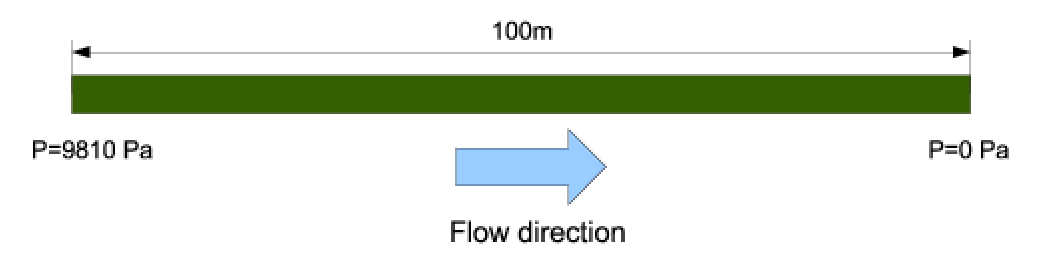
\includegraphics[scale=0.6]{FLUID_MOMENTUM/figures/oneDproblem.eps}
\end{center}
\caption{1D Flow Description}
\label{fm:1dflow}
\end{figure}


\item[Results:] No matter what element type is used for the problem, the pressure distribution and velocity field should be same as provied in Fig.\ref{fm:1d-result}.
%-------------------------------------------------
\begin{figure}[h]
\begin{center}
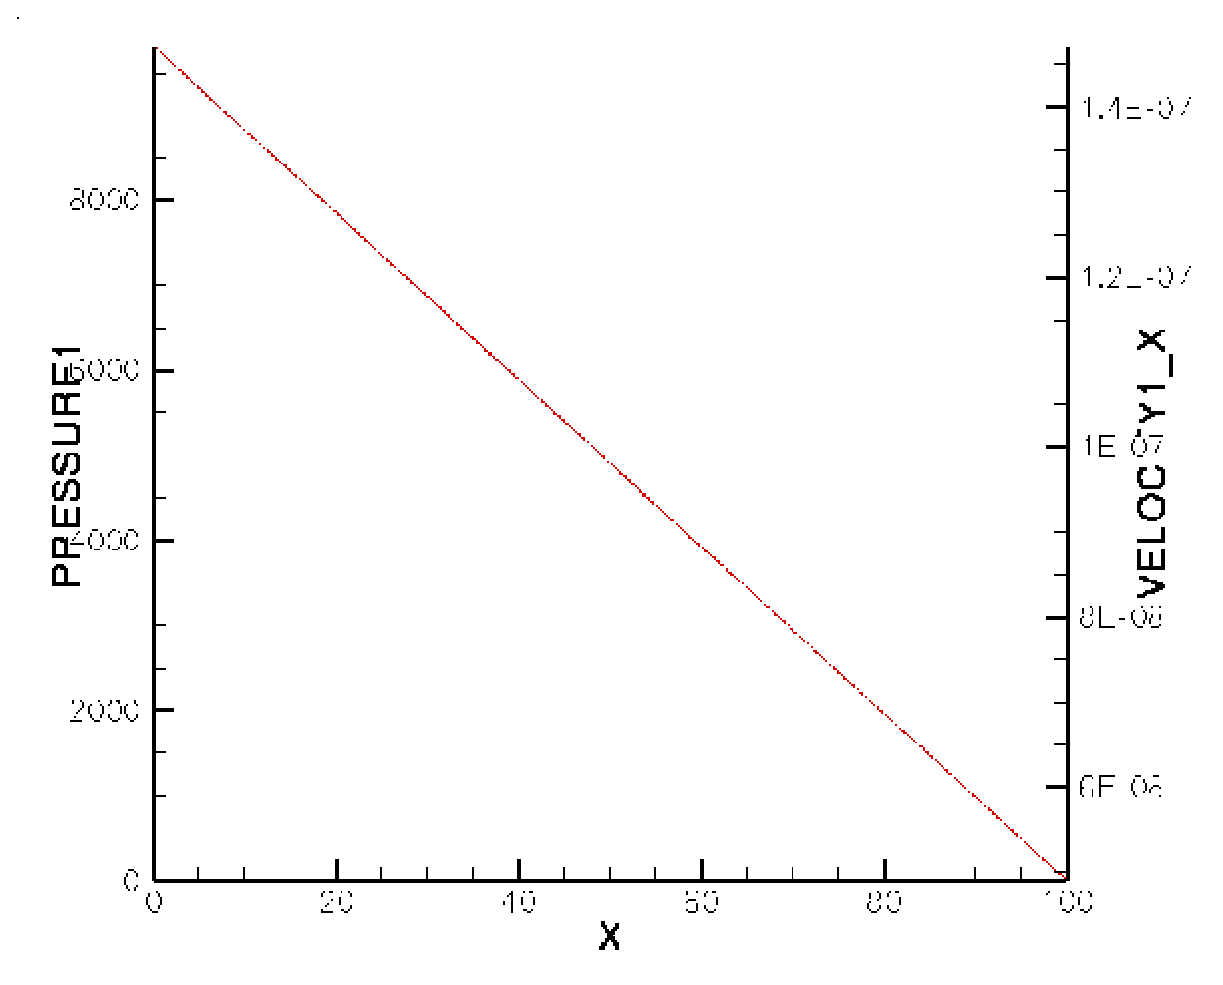
\includegraphics[scale=0.40]{FLUID_MOMENTUM/figures/1d-result.eps}
\end{center}
\caption{pressure and velocity}
\label{fm:1d-result}
\end{figure}


%-------------------------------------------------

\end{description}
